\label{sec:promotions-implementation}
PromotionsService.findValid dùng được với PrismaService khi xem trước và TransactionClient khi đặt hàng. calcDiscount/calcPoints là hàm thuần, tách quy tắc số học khỏi database để kiểm thử độc lập. OrdersService tạo dòng món theo giá backend, tính subtotal, kiểm voucher rồi lưu total/discount cùng đơn và snapshot kho trong một transaction.

LoyaltyService.award nhận cùng TransactionClient của thanh toán. Khi points dương, UPDATE User dùng increment nguyên tử, lấy số dư mới rồi ghi LoyaltyTransaction EARN. Payment, PAID, số dư và sổ điểm cùng commit hoặc cùng rollback; gửi lại kết quả đã xử lý không được gọi lại để cộng điểm thêm. Unique sổ điểm là lớp bảo vệ bổ sung, không thay thế kiểm settlement dưới khóa Order.

Hai đơn khác nhau cùng trả cho một User dùng phép increment tránh ghi đè số dư đọc cũ. Đổi bằng giá chỉ chuyển credit, không gọi award; đổi cao hơn gọi award qua thanh toán phần chênh lệch. Frontend đọc lại thông tin tài khoản sau kết quả thanh toán để hiển thị điểm do backend trả.

\begin{figure}[htbp]\centering
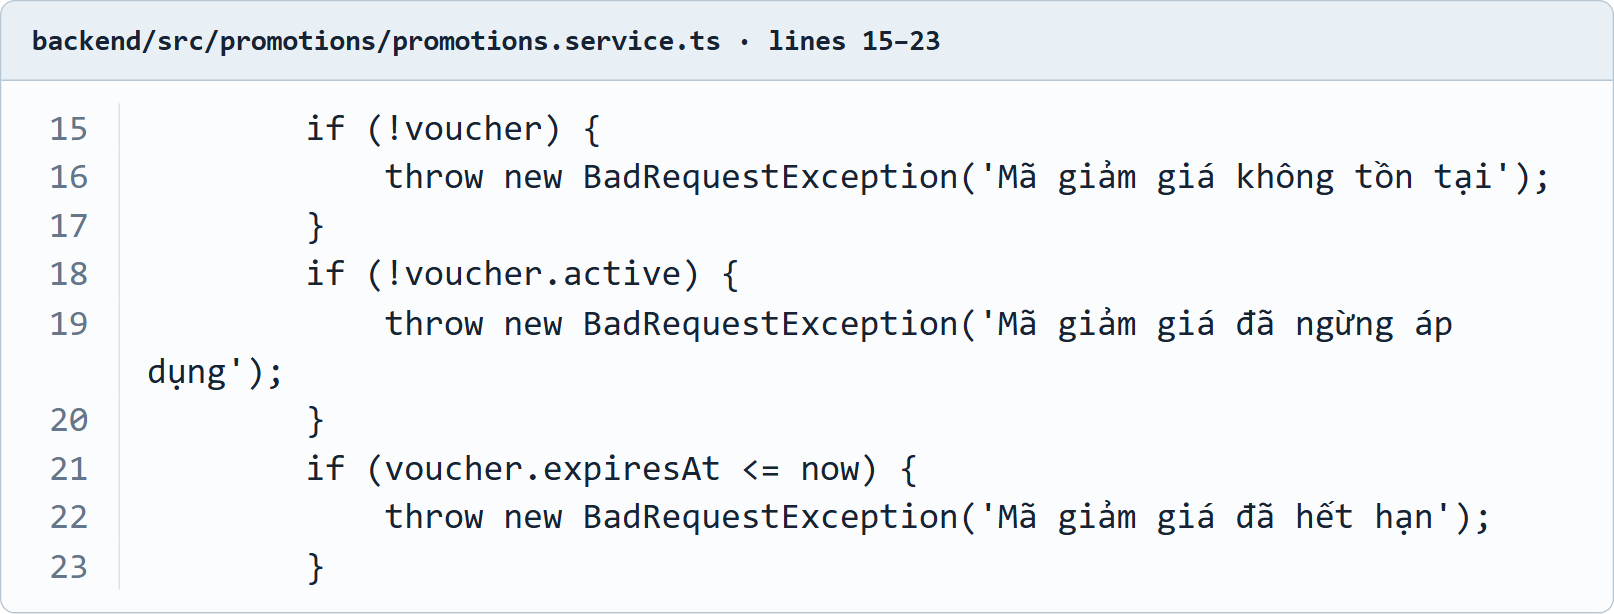
\includegraphics[width=.92\linewidth,height=.24\textheight,keepaspectratio]{assets/promotions/code-validation.png}
\caption{findValid kiểm mã, hiệu lực và hạn trước khi áp dụng}
\vspace{3mm}
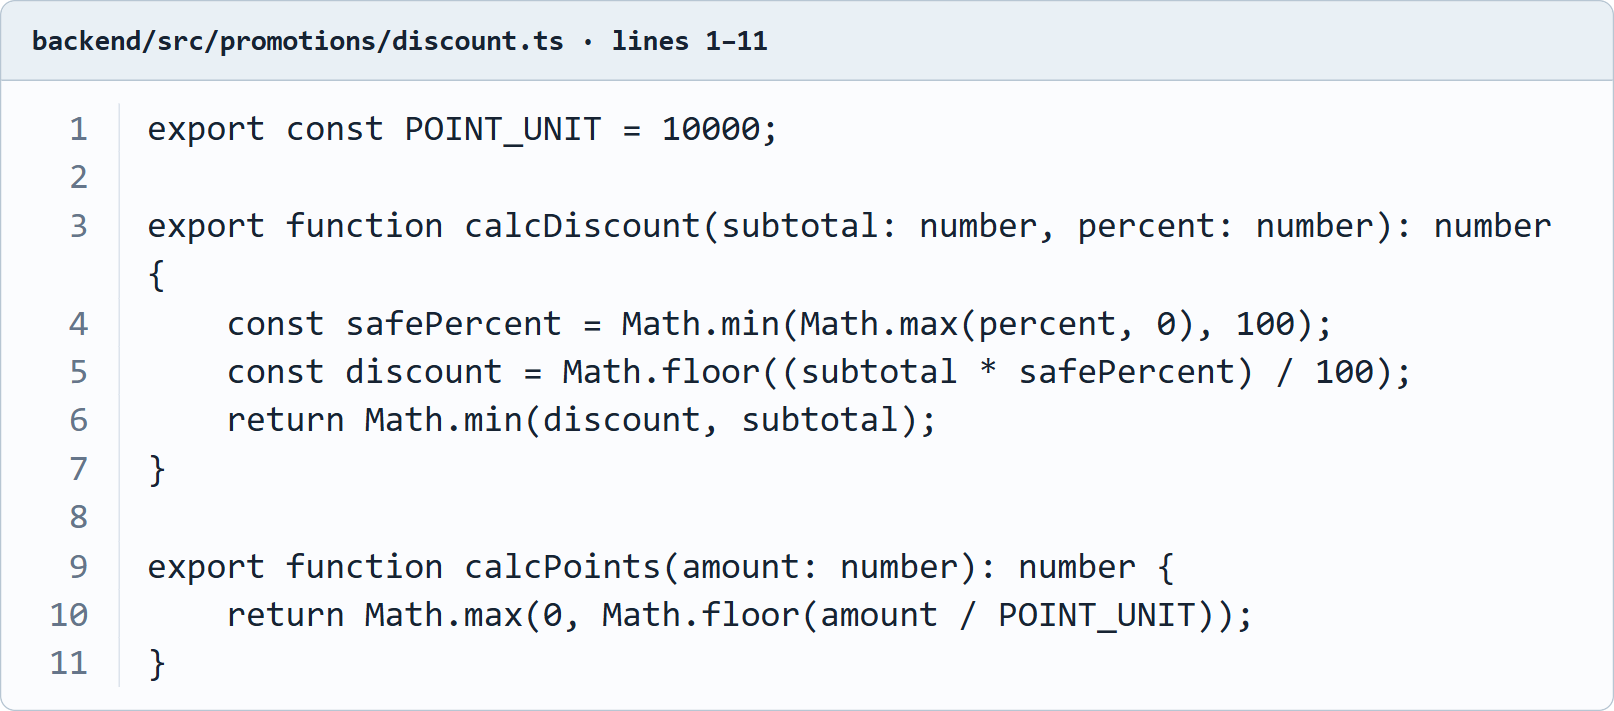
\includegraphics[width=.92\linewidth,height=.18\textheight,keepaspectratio]{assets/promotions/code-calculation.png}
\caption{Hai hàm thuần tính tiền giảm và điểm với quy tắc làm tròn}
\vspace{3mm}
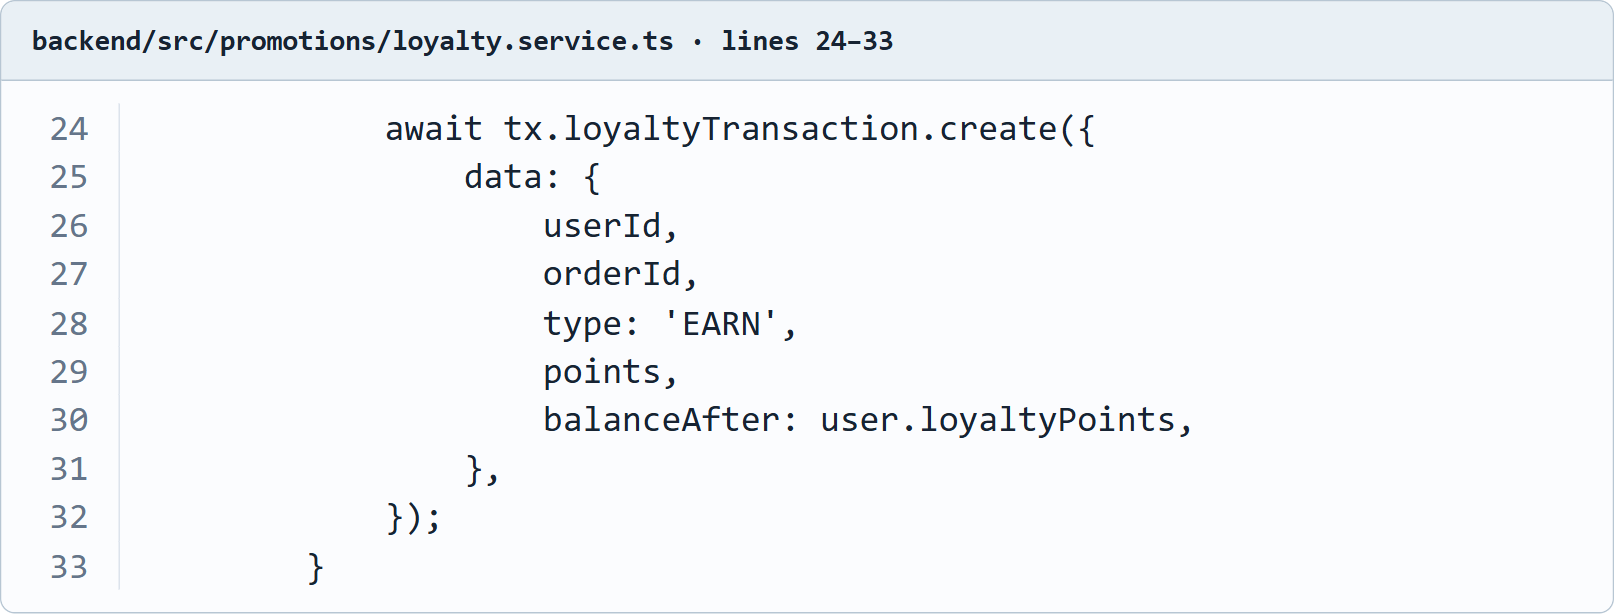
\includegraphics[width=.92\linewidth,height=.27\textheight,keepaspectratio]{assets/promotions/code-ledger.png}
\caption{award ghi EARN cùng số dư sau cập nhật trong transaction thanh toán}
\end{figure}
